\documentclass[aps,prd,onecolumn,showpacs,amsmath,amssymb,nofootinbib]{revtex4} \pdfoutput=1
 
\usepackage{amsfonts}
\usepackage{amsmath}
\usepackage{graphicx}
\usepackage{subfigure}
\usepackage{dcolumn}
\usepackage{bm}
\usepackage{booktabs}
\usepackage[utf8]{inputenc}
\usepackage{multirow}
\usepackage{graphicx,graphics,dcolumn,booktabs,bm}
\usepackage{longtable,lscape}
\usepackage{txfonts}
\usepackage{overpic}
\usepackage{amssymb}
\usepackage{indentfirst}
\usepackage{epsfig}
\usepackage{feynmf}   %{feynmp}
\usepackage{epstopdf}   %{feynmp}
\usepackage{slashed}  %for Feynman symbols
\usepackage{color}
\usepackage[section]{placeins}
\usepackage{svg}

\usepackage[colorlinks, citecolor=blue,anchorcolor=red,menucolor=red, linkcolor=red,filecolor=red,runcolor=red,urlcolor=blue,frenchlinks=red]{hyperref}



\usepackage{ulem}
\usepackage{physics}

\newcommand{\lsm}{L$\sigma$M}
\newcommand{\nlsm}{NL$\sigma$M}
\newcommand{\cpt}{$\chi$PT}
\newcommand{\groupsu}[1]{S\!U(#1)}
\newcommand{\gev}{\mathrm{GeV}}
\newcommand{\mev}{\mathrm{MeV}}



\begin{document}
\title{Models and Effective Theories of the Strong Interaction}

\author{J.~Ho}
\affiliation{Department of Physics and Engineering Physics\\ University of Saskatchewan\\ 
          Saskatoon, SK, S7N 5E2, Canada}

\begin{abstract}
We review the experimental status of the scalar meson states ($J^{P} = 0^{+}$) and discuss some of the experimental and theoretical challenges in uncovering their structure. We briefly review the importance of symmetries in constructing QCD, and introduce the linear and non-linear $\sigma$ models in the context of chiral symmetry. Chiral perturbation theory is motivated, and we discuss how these methods have been recently used in exploring properties of the scalar nonet.
\end{abstract}
\maketitle
\section{Introduction}\label{I}
While much interest and resources have been directed towards the TeV energy scales within particle physics as we search for answers regarding the Higgs, dark matter, and other fundamental questions, many open questions remain at low energy scales. In particular because of its fundamentally non-perturbative character, understanding quantum chromodynamics (QCD) and strong interactions at low energies presents experimental and theoretical challenges. We review the experimental status of the light hadronic spectrum focusing specifically on the controversy surrounding the scalar states and investigate some of the tools being used to explore the nature of these states, including linear and non-linear $\sigma$ models. This is by no means a comprehensive review of the literature; the scalar nonet is a long-standing open question in the hadronic physics community, and much work has been and is being done to understand the physics at these lower energies. 

\section{Low-energy QCD}\label{II}
\subsection{Experimental Background}
Below $2\,\mathrm{GeV}$, there exists a host of scalar hadronic resonances whose structure are unclear. While the higher energy vector and tensor states tend to be better understood, the scalar mesons are plagued with difficulties arising from wide resonance widths \& overlaps, cusps at mass thresholds, and the expectation of contamination by non-$\bar{q}q$ scalar states \cite{PDG2018}. While clearly defined flavour nonets of pseudoscalar and vector states can be formed from known states (Figures \ref{fig:meson-octet} and \ref{fig:vector-octet}), there exists an overpopulation of light scalars below an energy threshold of $2\,\gev$ to form a single nonet. It has been proposed that these states form two scalar flavour nonets: one of $q\bar q$ quarkonia, and one meson-meson or $qq\bar{q}\bar{q}$ nonet \cite{Jaffe1977,Close2002,tHooft2008}. Given the complexities in experimental analysis of low-lying scalar resonances such as the $f_0(500)$ or the $f_0(1370)$, support for this two nonet interpretation is not unanimous \cite{Ochs2001,Zhang2011}, with some suggesting that some of these higher energy resonances may be identified with excited quarkonium states \cite{Parganlija2017}. However, there are compelling reasons from our understanding of QCD that motivates a two octet model. A scalar glueball is predicted from QCD using several theoretical approaches; current methods put mass predictions in the range of $1.0\,\gev$ and $1.7\,\gev$ \cite{Mathieu:2008me,Ochs2013}, which makes some of the scalar states compelling candidates. While it is predicted that significant mixing occurs between the glueball and conventional scalar meson states, details about the dynamics of the glueball are not yet understood. However, it is predicted that mixing with scalar meson states will manifest in three particular combinations aligning with the observations of the $f_0(1500)$, $f_0(1370)$, and $f_0(1710)$ states. Below $1\,\gev$ we expect the behaviour of quark interactions to be different that in the perturbative regime. In particular, it is predicted that the interaction between diquark pairs becomes more significant \cite{Jaffe1977}, very similar to the meson-meson attraction at low energies. Additionally, the observed inverted hierarchy in the mass spectrum observed below $1\,\gev$ suggests a structure outside the conventional quark model; when examining the masses and isospin for what is strongly suggested to be the lowest-lying scalar nonet ($f_0(500)$, $K_0^{*}(700)$, $a_0(980)$, and $f_0(980)$), states with strange quark content ($K_0^{*}(700)$) have lighter masses than states with no strange quark content ($a_0(980)$). This is contrary to what is anticipated in a $q\bar q$ system, with some suggesting these states represent the formation of a $qq\bar{q}\bar{q}$ or meson-meson nonet  \cite{Jaffe1977, Pelaez2011}.  

The nature of these hadronic states above and below $1\,\gev$ is far from settled, and more experimental investigation is necessary to clarify the picture. While these resonances have long been observed experimentally, many of them are not well understood given their overlapping or large widths, proximity to thresholds, and susceptibility to glueball mixing. What follows is a brief review of the status of each isospin group of the $J^{PC}=0^{++}$ resonances in the literature. 

\subsubsection{$a_{0}(980)$ and $a_{0}(1450)$}
The $a_0$ isovector states ($I=1$), $a_{0}(980)$ and $a_{0}(1450)$, are both well-established experimentally \cite{Abele1998}, but conclusions as to their structure have yet to be confirmed. The $a_{0}(980)$ state exists just below the $\bar K K$ threshold manifesting as a cusp between the $K\bar K$ and $\pi \eta$ channels \cite{Uehara2002}, making it difficult to accurately determine its resonance width (Table \ref{table:scalars}). Because of its position so close to the $K \bar K$ threshold, many models suggest it is a four-quark state \cite{Jaffe1977,Liu1981,Giacosa2008,Achasov2010,Zhang2011}, and this interpretation is consistent with two-photon, $\phi$, and $J/\psi$ decays \cite{Barnes1985, Achasov2006}. Alternatively, some have suggested that the $a_0(980)$ state is the lowest-lying $q\bar q$ state \cite{Narison2000,Zhang2011}, while the $a_0(1450)$ represents a first excited state \cite{Zhang2011}. If the $a_0(980)$ is indeed a four-quark state, this begs the question as to whether the remaining $a_{0}(1450)$ state corresponds to the isovector scalar $q\bar q$ state, given that its heavier mass compared to $a_{0}(980)$ is inconsistent with the conventional quark model predictions \cite{Pelaez2011} . In the large $N_c$ expansion, the $a_0(1450)$ is consistent with $q\bar q$ quarkonium \cite{Giacosa2008}. Calculations from lattice QCD indicate the $a_0(1450)$ is consistent with a conventional $q\bar{q}$ state \cite{Mathur2007}, while the $a_0(980)$ is not \cite{McNeile2006,Mathur2007}, however it appears that more recent lattice calculations contradict this \cite{Alexandrou2013,Wagner2013}. 

\subsubsection{$K^{*}_{0}(700)$ and $K^{*}_{0}(1430)$}
Comprising the $I = 1/2$ states are the $K^{*}_{0}(700)$ and $K^{*}_{0}(1430)$. The PDG considers the $K^{*}_{0}(1430)$ to be the most well-established of the light scalar mesons \cite{PDG2018}. The observation of mass and resonance width is consistent with predictions from chiral perturbation theory. From theoretical calculations in QCD sum rules \cite{Narison2000,Du2005}, the $K^{*}_{0}(1430)$ is predicted to be a conventional $s\bar{q}$ or $q\bar{s}$ state ($q$ denoting a $u$ or $d$ quark). Lattice QCD calculations are not clear, with contradicting predictions as to the nature of both the $K^{*}_{0}(700)$ and $K^{*}_{0}(1430)$ \cite{Prelovsek2010,Alexandrou2013}. Methods employing a large $N_c$ expansion indicate that $K^{*}_{0}(700)$ is consistent with a four-quark state, while $K^{*}_{0}(1430)$ is a $q\bar q$ resonance \cite{Giacosa2008}.
Historically known as the $\kappa$, the $K^{*}_{0}(700)$ resonance has a large width, similar to the $f_0(500)$ meson discussed later on. This width, as well as its close proximity to the $K\pi$ threshold make it difficult to observe experimentally.

\subsubsection{$f_0$ states}
The $f_0$ states ($I=0$) constitute a wide ranging class of observed resonances, some better established than others, with no clear structural assignment. The $f_0(980)$ has been categorized as a both a member of the $q\bar{q}$ scalar nonet \cite{Tornqvist1996,Shi1999} as well as that of a four-quark nonet \cite{Black1999,Markushin2000,Fariborz2003}, with \cite{Fariborz2003} indicating a large glueball component in the state. An analysis of two-photon decay widths indicate the $f_0(980)$ can be interpreted predominantly as a $K\bar{K}$ molecular state \cite{Lemmer2007}, while conclusions from QCD sum rules claims the opposite \cite{Lee2013}. In recent observations of $B$-decays \cite{Aaij2014,Daub2015}, we also see conflicting conclusions as to the nature of the $f_0(980)$ structure; while the LHCb collaboration excludes a tetraquark interpretation of the $f_0(980)$ to an $8\sigma$ level in a model-dependant analysis \cite{Aaij2014}, a different model-independent analysis of the same data suggests otherwise \cite{Daub2015}.  Clearly the nature of this state is far from decided, and much more experimental and theoretical work is needed to discern its structure.

A consequence of the non-abelian nature of QCD is in the dynamics of the bicolored gluons and the possibility of the formation of pure gluon bound states, also known as glueballs. While not explicitly part of the scalar nonet, it is predicted that a scalar glueball ($J^{PC} = 0^{++}$) exists at energies between $1.0\,\gev$ and $1.7\,\gev$ \cite{Ochs2013}, which makes identification of other scalar states at this energy complicated as it is anticipated that these glueballs will mix with $q\bar q$ states. No conclusive observation of this glueball state has been recorded, but there are predictions that it could be identified in the scalar resonances shown here in Table \ref{table:scalars}. Specifically, the $f_0(1370)$, $f_0(1500)$, and $f_0(1710)$ states have all been suggested as possible glueball candidates \cite{Ochs2013, Fariborz2003,Janowski2011}. Given the possibility of mixing, some or all of these states could contain a glueball component. Calculations from lattice QCD and QCD sum rules are inconclusive, with some favoring a scalar glueball around $\approx 1.7 \,\gev$ \cite{Gui2012,Huang1999,Yuan:2009vs}, and others around $1.3\,\gev$ \cite{FORKEL2004}. A recent review of lattice, sum rule, and constituent models assess the approximate scalar glueball predictions from a compilation of the literature as follows: $1.7\,\gev$ (lattice), $1.25\,\gev$ (QCD sum rules), $1.6\,\gev$ (AdS/CFT), and $1.3\,\gev$ (Bag model) \cite{Mathieu:2008me}. An analysis of $J/\psi$ decay data from BES indicates that the data is consistent with mixing between the $f_0(1370)$, $f_0(1500)$, and $f_0(1710)$ states, with $f_0(1370)$ carrying dominantly $q\bar q$ character, $f_0(1710)$ dominantly $s \bar s$, and the $f_0(1500)$ dominantly glueball. With other many interpretations and mechanisms proposed in the literature that further complicate the picture \cite{Janowski:2014ppa,Albaladejo2008}, the future status of the glueball in the context of the $f_0$ resonances remains murky. Experiments such as GlueX \cite{Gutsche2016} will hopefully shed some light on whether some or all of these scalar states carry a glueball component.

\subsubsection{The $f_0(500)$ meson}
Perhaps the most historically controversial particle, the $f_0(500)$ meson (known first and most widely as the $\sigma$ meson) was first theoretically born in the proposed linear $\sigma$ model, where a scalar singlet was introduced to preserve chiral symmetry in Gell-Mann and L\'evy's original effective model for the strong interaction between nucleons and pions \cite{GellMann1960}. A relatively light scalar meson was proposed by Teller and Johnson \cite{Teller1955} and embraced by Schwinger \cite{Schwinger1957} as a possible unstable scalar state which he named the $\sigma$, after which it was incorporated by Gell-Mann and L\'evy into their models. Over the next 16 years, candidates for the $\sigma$ would come and go from the literature under different names including the $\epsilon$ or $\eta_{0+}$ \cite{Pelaez2011}, finally disappearing from the literature until 1996 \cite{Tornqvist1996} when careful reanalyses of the $\pi\pi$ S-wave scattering data showed an unstable, wide resonance which was named the $f_0(400-1200)$, reflecting its large mass uncertainty\cite{Pelaez2011}. Since it was established in the Review of Particle Properties \cite{Barnett1996}, it has most recently been renamed $f_0(500)$, with significantly reduced uncertainties in mass and widths (Table \ref{table:scalars}). It is an unusual resonance in the sense that it is as wide as it is heavy, it is not appropriately modelled by the conventional Breit-Wigner resonance shape and, as Schwinger predicted, it is very unstable. These all contribute to making it a difficult resonance to experimentally observe with precision. 


%Theoretical NJL mass prediction \cite{Schumacher2011} $m_{\sigma} = 0.685\,\gev$


\begin{table}[!htb]
\begin{tabular}{|c|c|c|c|c|}
\hline

PDG Reference   & Alias(es) & $I(J^{PC})$     & Mass ($\gev$) & Width ($\gev$) \\ 
$K^{*}_0(700)$  & $\kappa$  & $\frac{1}{2}(0^{+})$ &  $0.824\pm0.030$  &    $0.478\pm0.050$            \\
$K^{*}_0(1430)$ &           & $\frac{1}{2}(0^{+})$ & $1.425\pm0.050$ & $0.270\pm0.080$             \\ 
$a_0(980)$      &     $\delta(976)$      & $1(0^{++})$           & $0.980\pm0.020$ & $0.050-0.100$               \\ 
$a_0(1450)$     &           & $1(0^{++})$           & $1.474\pm0.019$ & $0.265\pm0.013$             \\ 
$f_0(500)$      & $\sigma$, $\epsilon(700)$, $\eta_{0+}$  & $0(0^{++})$     & $0.400 - 0.550$ & $0.400 - 0.700$               \\ 
$f_0(980)$      &           & $0(0^{++})$           & $0.990\pm0.020$ & $0.040-0.100$               \\ 
$f_0(1370)$     &           & $0(0^{++})$           & $1.200-1.500$   & $0.200-0.500$               \\
$f_0(1500)$     &           & $0(0^{++})$           & $1.505\pm0.006$ & $0.109\pm0.007$             \\ 
$f_0(1710)$     &           & $0(0^{++})$           & $1.722^{+0.006}_{-0.005}$ & $0.135\pm0.007$               \\ \hline
\end{tabular}
\caption{Summary of experimental data on scalar mesons observed below $2\,\gev$ \cite{PDG2018}.}
\label{table:scalars}
\end{table}

% The masses of these scalar mesons seem to indicate a structure distinct from that of the vector or tensor mesons (see Figure \ref{}); the reversed mass hierarchy is consistent with a four-quark ($qq\bar{q}\bar{q}$) interpretation rather than a $q\bar{q}$ structure \cite{Fariborz2010,Jaffe1977}, which has lead many researchers to believe the lowest-lying scalar nonet to be formed exclusively of four-quark states \cite{Schumacher2011,Tornqvist2002,Close2002,Fariborz2009}. 

\subsection{Symmetries}
%We know now that hadrons are made up of constituent quarks, and because of colour confinement free quarks are not observed; historically, much of the investigation into hadronic structure had to be done implicitly. Much of our understanding of the strong interaction was developed before the notion of quarks and gluons was even conceptualized; by examining mathematical symmetries of the Lagrangians and equations of motion, deep insights can be made into the nature of matter. Emmy Noether's insight into how continuous symmetries in nature translate into conserved quantities was a revolutionary shift that has enormously impacted how we approach modern physics. She stated that...[MATHS HERE]. Her ideas form the foundation of many of the most important insights into particle physics to date.

Symmetries play a vital role in developing models and effective theories for explaining physical phenomena. We know from the work of Emmy Noether that continuous symmetries correspond with conserved currents. More formally, this can be expressed in the following way: given an infinitesimal transformation of a field $\phi$ 
\begin{equation}
    \label{noetherTransformation1}
    \phi_{i}(x) \rightarrow {\phi'}_{i}(x) = \phi_{i}(x) + \delta \phi_{i}(x),
\end{equation}
for
\begin{equation}
    \label{noetherTransformation2}
    \delta \phi_{i}(x) = -i \Theta^{a} T^{a}_{ij}\phi_{j}(x),
\end{equation}
where $\Theta \in \mathbb{R}$ and $T^{a}$ are matrices satisfying the Lie algebra of the group representing a symmetry, if the Lagrangian is invariant under that symmetry there is a conserved Noether current given by
\begin{equation}
    \label{noetherTheorem}
    \partial^\mu j_{\mu}(x) = 0
\end{equation}
where
\begin{equation}
    \label{noetherCurrent}
    j^{a}_{\mu} = -i \frac{\partial\mathcal{L}}{\partial\left(\partial^{\mu}\phi_{i}\right)}T^{a}_{ij}\phi_{j}(x)
\end{equation}

Experimentally, we have found that hadrons are made up of constituent quarks, and because of colour confinement free quarks are not observed; historically, the prediction of quarks and investigation into hadronic structure was done through the examination of symmetries, such as in the classification of the pseudoscalar and vector nonets in Gell-Mann's ``Eightfold Way'' \cite{GellMann1962} shown in Figures \ref{fig:meson-octet} and \ref{fig:vector-octet}. Gell-Mann observed the pseudoscalar mesons to fit into an \groupsu{3} symmetry, leading to the prediction of the light quarks ($u$, $d$, and $s$) as constituent particles \cite{GellMann1964, Zweig1964}.
\begin{figure}[!ht]
    \centering
    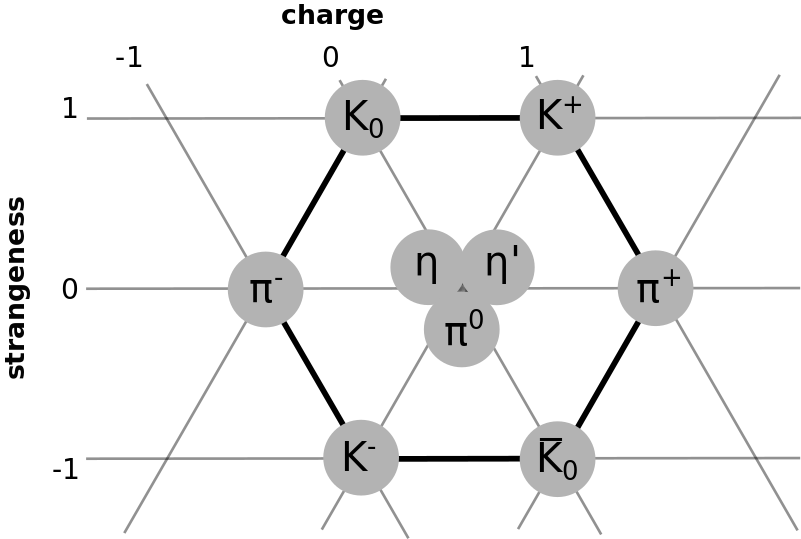
\includegraphics[scale=0.5]{octet.png}
    \caption{Pseudoscalar Octet}
    \label{fig:meson-octet}
\end{figure}

\begin{table}[!htb]
\begin{tabular}{|c|c|c|c|c|c|}
\hline
Meson       & Quark Content                                                                                  & Isospin, $I$  & Charge & $J^{P(C)}$ & \begin{tabular}[c]{@{}l@{}}Mass ($\mev$)\end{tabular}     \\

$\pi^{0}$   & $\frac{1}{\sqrt{2}}\left(u\bar{u}-d\bar{d}\right)$                                             & 1             & 0      & $0^{-+}$   & $134.9770\pm0.0005$                                          \\
$\pi^{+}$   & $u\bar{d} $                                                                                    & 1             & +1     & $0^-$      & $139.57061\pm0.00024$                                        \\
$\pi^{-}$   & $d\bar{u} $                                                                                    & 1             & -1     & $0^-$      & $139.57061\pm0.00024$                                        \\
$K_0$       & $d\bar{s}$                                                                                     & $\frac{1}{2}$ & 0      & $0^-$      & $497.611\pm 0.013$                                           \\
$\bar{K}_0$ & $s\bar{d}$                                                                                     & $\frac{1}{2}$ & 0      & $0^-$      & $497.611\pm 0.013$                                           \\
$K^{+}$     & $u\bar{s}$                                                                                     & $\frac{1}{2}$ & +1     & $0^-$      & $493.677\pm0.016$                                            \\
$K^{-}$     & $s\bar{u}$         & $\frac{1}{2}$ & -1     & $0^-$      & $493.677\pm 0.016$ \\
$\eta$      & $\frac{1}{\sqrt{3}}(u\bar{u}+d\bar{d}-2s\bar{s})$                                              & 0             & 0      & $0^{-+}$   & $547.862\pm0.017$                                            \\
$\eta'$     & $\frac{1}{\sqrt{6}}(u\bar{u}+d \bar{d}+s\bar{s} )$ & 0             & 0      & $0^{-+}$   & $957.78\pm0.06$              \\
\hline
\end{tabular}
\caption{Properties of the pseudoscalar octet depicted in Figure \ref{fig:meson-octet} \cite{PDG2018}.}
\label{table:pseudoscalars}
\end{table}

\begin{figure}[!ht]
    \centering
    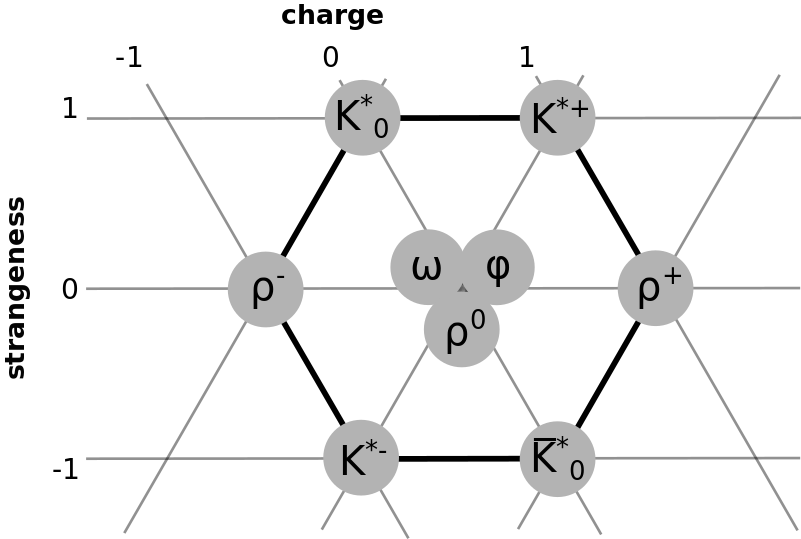
\includegraphics[scale=0.5]{vector-octet.png}
    \caption{Vector Octet}
    \label{fig:vector-octet}
\end{figure}
\begin{table}[!htb]
\begin{tabular}{|c|c|c|c|c|c|}
\hline
Meson                & Quark Content                                      & Isospin, $I$  & Charge & $J^{P(C)}$                                             & \begin{tabular}[c]{@{}l@{}}Mass ($\mev$)\end{tabular} \\
$\rho^{0}(770)$      & $\frac{1}{\sqrt{2}}\left(u\bar{u}-d\bar{d}\right)$ & 1             & 0      & $1^{--}$                                               & $775.26\pm0.25$                                          \\
$\rho^{+}(770)$      & $u\bar{d} $                                        & 1             & +1     & $1^{-}$                                                & $775.11\pm0.34$                                          \\
$\rho^{-}(770)$      & $d\bar{u} $                                        & 1             & -1     & $1^{-}$                                                & $775.11\pm0.34$                                          \\
$K^{*}_0(892)$       & $d\bar{s}$                                         & $\frac{1}{2}$ & 0      & $1^{-}$                                                & $895.55\pm 0.20$                                         \\
$\bar{K}^{*}_0(892)$ & $s\bar{d}$                                         & $\frac{1}{2}$ & 0      & $1^{-}$ & $895.55\pm 0.20$                                         \\
$K^{*+}(892)$        & $u\bar{s}$                                         & $\frac{1}{2}$ & +1     & $1^{-}$  & $891.76\pm0.25$                                          \\
$K^{*-}(892)$        & $s\bar{u}$                                         & $\frac{1}{2}$ & -1     & $1^{-}$  & $891.76\pm0.25$                                          \\
$\omega(782)$        & $\frac{1}{\sqrt{2}}(u\bar{u}+d\bar{d})$            & 0             & 0      & $1^{--}$ & $782.65\pm0.12$                                          \\
$\phi(1020)$         & $s\bar{s}$                                         & 0             & 0      & $1^{--}$ & $1019.461\pm0.019$  \\
\hline
\end{tabular}
\caption{Properties of the vector octet depicted in Figure \ref{fig:vector-octet} \cite{PDG2018}.}
\label{table:vectors}
\end{table}
\begin{figure}
    \centering
    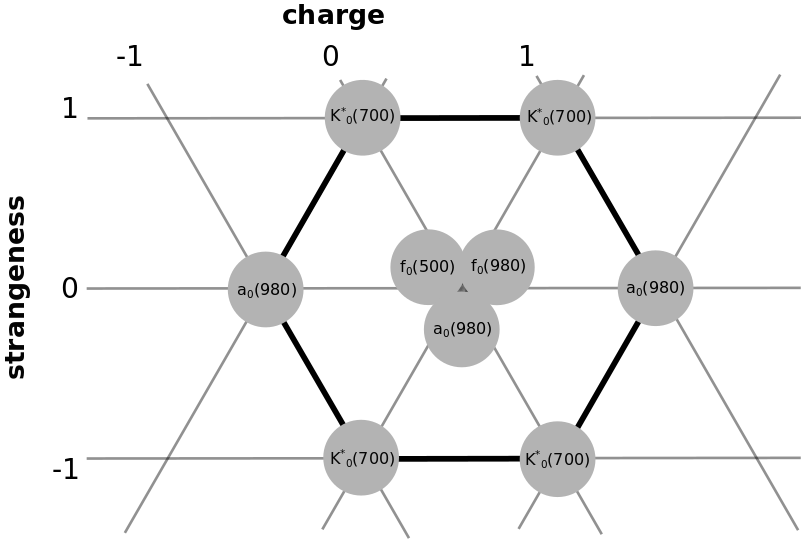
\includegraphics[scale=0.5]{scalar-octet.png}
    \caption{Proposed scalar octet from Ref. \cite{Jaffe1977} with updated particle identification.}
    \label{fig:scalar-octet}
\end{figure}
As important to examine are the deviations from symmetries that we see in nature, also known as symmetry breaking. Symmetry breaking in quantum field theories manifests in three different ways:
\begin{itemize}
    \item Explicit symmetry breaking
    \item Spontaneous symmetry breaking
    \item Anomalous (quantum mechanical) symmetry breaking
\end{itemize}
QCD contains examples of all three of these. We will find that the QCD Lagrangian carries an approximate $S\!U_{L}(N_f)\times S\!U_{R}(N_f)$ chiral symmetry that is both explicitly broken by the mass terms in the Lagrangian, as well as spontaneously broken from $S\!U_{L}(N_f)\times S\!U_{R}(N_f) \rightarrow S\!U_{V}(N_f)$ generating three pseudo-Nambu-Goldstone bosons. We will not focus our discussion on the anomolously broken $U_{A}(1)$ abelian axial symmetry in QCD; though it appears as a classical symmetry, it is broken in the quantum theory, generating terms in the Lagrangian that violate $CP$ symmetry. This is also known as the strong $CP$ problem.

\subsubsection{Explicit Symmetry Breaking and Chiral Symmetry}
Consider the the QCD Lagrangian
\footnote{$G^{a}_{\mu \nu}\left(x\right) = \partial_{\mu}B_{\nu}^{a}\left(x\right)-\partial_{\nu}B_{\mu}^{a}\left(x\right)+g f^{abc} B_{\mu}^{b}\left(x\right) B_{\nu}^{c}\left(x\right)$, and $\slashed{D} = D^{\mu}\gamma_{\mu} = (\partial^{\mu}-i g t_{a} B^{\mu}_{a}\left(x\right)) \gamma_{\mu}$}
\begin{equation}
\mathcal{L}_\mathrm{QCD}=  \bar{\psi}(i\slashed{D}-m)\psi-\frac{1}{4}\left(G^{a}_{\mu \nu}\right)^2.
\label{qcdlagrangian}
\end{equation}

and introduce the left- and right-handed chiral fields
\begin{gather}\label{chiralFields}
    \psi_{L} = \Gamma_{L}\psi\\
    \psi_{R} = \Gamma_{R}\psi\\
    \psi = \psi_{L} + \psi_{R}
\end{gather}
where
\begin{gather}\label{chiralOperators}
    \Gamma_{L} = \frac{1}{2}(1+\gamma_{5})\\
    \Gamma_{R} = \frac{1}{2}(1-\gamma_{5}).
\end{gather}

We note that our chiral operators \eqref{chiralOperators} have the properties 
\begin{gather}
    \Gamma_{L} + \Gamma_{R} = 1\\
    \Gamma_{L,R}\Gamma_{L,R} = \Gamma_{L,R}\\
    \Gamma_{L}\Gamma_{R}= \Gamma_{R}\Gamma_{L} = 0.
\end{gather}
The Lagrangian \eqref{qcdlagrangian} then takes the form
\begin{equation}
    \label{chiralqcdLagrangian}
    \mathcal{L}_\mathrm{QCD}^\mathrm{chiral} = \bar{\psi}_{L}i\slashed{D}\psi_{L}+\bar{\psi}_{R}i\slashed{D}\psi_{R}-(\bar{\psi}_{L} m \psi_{R}+\bar{\psi}_{R} m \psi_{L})-\frac{1}{4}\left(G^{a}_{\mu \nu}\right)^2.
\end{equation}
Notice that the mass terms in \eqref{chiralqcdLagrangian} couple the $\psi_{L}$ and $\psi_{R}$ fields, and without these terms the Lagrangian would be invariant under the global symmetries
\begin{equation}\label{chiralSymmetries}
    \psi_{L,R} \rightarrow \exp(-i \alpha_{L,R}) \psi_{L,R}\quad (\alpha_{L,R} \in \mathbb{R}).
\end{equation}
The mass term in the Lagrangian \eqref{chiralqcdLagrangian} spoils the chiral symmetry \eqref{chiralSymmetries}; this is \textit{explicit symmetry breaking} in QCD. However, in theory and experiment taking the chiral limit ($m \rightarrow 0$) is a good approximation for the light quarks $u,\,d$; this establishes a ${S\!U}_L(2)\times {S\!U}_R(2)$ chiral symmetry. If we include the strange quark $s$, this extends the symmetry to ${S\!U}_L(3)\times {S\!U}_R(3)$, although given the significant mass difference between the $u,\,d$ and $s$ quarks, the symmetry remains a decent approximation relative to the energy scale of QCD ($\approx 1\,\gev$). It is from this ${S\!U}_L(3)\times {S\!U}_R(3)$ symmetry that the nonet representations in Figures \ref{fig:meson-octet} and \ref{fig:vector-octet} emerge. 
We can explore this chiral symmetry further using Noether's theorem \eqref{noetherTheorem} and \eqref{noetherCurrent}. From the chiral expression of the QCD Lagrangian \eqref{chiralqcdLagrangian}, we can find the corresponding Noether currents
\begin{gather}
    \label{chiralnoethercurrents}
    j_{L}^{\mu} = \bar{\psi}_{L}\gamma^\mu \psi_{L}\\
    j_{R}^{\mu} = \bar{\psi}_{R}\gamma^\mu \psi_{R},
\end{gather}
which combine to form the vector ($V^\mu$) and axial vector ($A^\mu$) currents 
\begin{gather}
   V^\mu = j_{L}^{\mu} + j_{R}^{\mu} = \bar{\psi} \gamma^{\mu} \psi \label{vectorcurrent}\\
   A^\mu = j_{L}^{\mu} - j_{R}^{\mu} = \bar{\psi} \gamma_{5}\gamma^{\mu} \psi.
   \label{axialvectorcurrent}
\end{gather}
 From these combinations, we can see that the chiral symmetry ${S\!U}_L(N_f)\times {S\!U}_R(N_f)$ is related to the vector and axial vector symmetries corresponding to the same dimensions (in this case, ${S\!U}_V(2)\times {S\!U}_A(2)$)\footnote{This is an abuse of notation; while ${S\!U}_V(2)$ is a subgroup of ${S\!U}_L(N_f)\times {S\!U}_R(N_f)$, the axial transformations do not form a subgroup \cite{Pelaez2011}}. Returning for a moment to consider the case where $m \neq 0$, we can confirm our understanding of the explicit symmetry breaking of the axial current by the nonzero quark masses. From \eqref{vectorcurrent} and \eqref{axialvectorcurrent} and the Dirac equation, it follows that
 \begin{gather}
     \label{vectorcurrentdivergence}
     \partial_\mu V^{\mu} = 0\\
     \label{axialvectorcurrentdivergence}
     \partial_\mu A^{\mu} = 2 i m \bar{\psi} \gamma_{5} \psi .
 \end{gather}
 We observe that in the chiral limit, the axial vector current is conserved; the axial vector component of the chiral symmetry is explicitly broken through the mass terms in the Lagrangian.
%The vector and axial vector transformations are
% \begin{gather}\label{vectorSymmetries}
%     \psi \rightarrow \exp(i \theta^{a}_{V} t^{a}) \psi\\
%     \psi \rightarrow \exp(i \gamma_{5}\theta^{a}_{A} t^{a}) \psi
% \end{gather}
\subsubsection{Spontaneous Symmetry Breaking and Nambu-Goldstone Bosons}
Formally, spontaneous symmetry breaking in the Nambu-Goldstone realization is defined by the condition
\begin{equation}\label{eq:ssb}
    \bra{0} \left[ Q_{a},\mathcal{O}_{i}\right]\ket{0} = -(T_{a})_{ij}\bra{0}\mathcal{O}_{j}\ket{0}\neq 0,
\end{equation}
where $(T_{a})_{ij}$ is the generator associated with the continuous symmetry, and $\mathcal{O}_i$ are a set of field operators. Eq. \eqref{eq:ssb} illustrates that a spontaneously broken symmetry manifests when a generator of a continuous symmetry fails to annihilate the vacuum state. Conceptually speaking, we can say that spontaneous symmetry breaking occurs if the ground-state of the field $\mathcal{O}_{i}$ does not carry the same symmetries as the vacuum; this corresponds to the ubiquitous double-well analogy (see discussions in Section \ref{III} for more details). If we consider a Lagrangian with a rotational symmetry, spontaneous symmetry breaking can be imagined as depicted in Figure \ref{fig:ssb}. 
\begin{figure}[!ht]
    \centering
    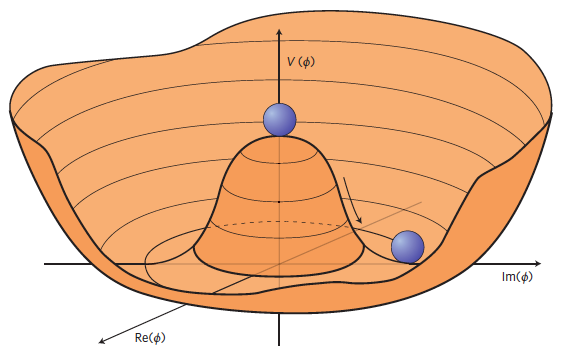
\includegraphics[scale=0.5]{higgspotential.png}
    \caption{Spontaneous symmetry breaking double-well potential \cite{doi:10.1142/9789814733519_0014}.} 
    \label{fig:ssb}
\end{figure}
We see that the Lagrangian (or more specifically in this case, the potential term of the Lagrangian) carries rotational symmetry, however a particle in its ground state would not carry the same rotational symmetry. This is the manifestation of spontaneous symmetry breaking.

There is strong evidence to support the idea that spontaneous symmetry breaking occurs in QCD. The mesons in the pseudoscalar octet are unnaturally light when compared with the vector octet, with a mass difference that cannot be generally explained by the difference in quark content. This is a manifestation of Nambu-Goldstone bosons, an important signal of spontaneous symmetry breaking. With each broken generator in \eqref{eq:ssb}, a massless scalar boson is generated. However, given that the chiral symmetry in QCD is only \textit{partially} conserved due to explicit symmetry breaking coming from the light quark masses, the pions still carry some mass, but are drastically lighter than expected. We can examine the patterns of known mesons in Tables \ref{table:pseudoscalars} and \ref{table:vectors}, and see a large disparity in mass between the lowest lying pseudoscalars and the vector mesons. The $\pi^0$ meson carries a mass of $\approx 135\,\mev$ while the vector of the same quark content, the $\rho^{0}$ has a mass of $\approx 775\,\mev$, a difference of over $600\,\mev$. We also do not see nearly the same disparity between heavy quark analogues; this points to something unique happening in the light quark sector. The pseudoscalar mesons are the Nambu-Goldstone bosons of the chiral symmetry breaking in QCD, with the pions being the best example of Nambu-Goldstone bosons, given that they are made up of the lightest quarks. Because the pseudoscalar are not truly massless bosons, they are often described as \textit{pseudo-}Nambu-Goldstone bosons. 

Another sign that spontaneous symmetry breaking is occuring in QCD comes from the vector ($J=1$) states. As both the vector \eqref{vectorcurrent} and axial vector \eqref{axialvectorcurrent} currents are conserved in the chiral limit, we would expect vector and axial vector multiplets to be observed at similar mass scales; in other words, we expect two meson multiplets with opposite parities ($P=\pm1$) to emerge at comparable energies. However, we find that the lightest $J^P = 1^{-}$ vector state $\rho(770)$ is $400\,\mev$ lighter than the lightest $J^P=1^{+}$ axial vector state observed, the $h_{1}(1170)$. This indicates that in QCD, it is the axial symmetry is also broken through spontaneous symmetry breaking, and ${S\!U}_L(N_f)\times {S\!U}_R(N_f)$ spontaneously breaks down to the vector subgroup, ${S\!U}_V(N_f)$.

Finally, under spontaneous symmetry breaking we expect to find a non-vanishing vacuum expectation value emerging as expressed in \eqref{eq:ssb}. But what is the operator $\mathcal{O}_j$ associated with the spontaneous breaking of chiral symmetry? Because we associate this expectation value with the vacuum, we require it satisfy the symmetry of the vacuum; it must be a Lorentz scalar, a colour singlet, and be non-invariant under the broken ${S\!U}_L(N_f)\times {S\!U}_R(N_f)$ symmetry, yet invariant under ${S\!U}_V(N_f)$. The lowest dimensional candidate that we can build from QCD is what is referred to as the \textit{chiral condensate},
\begin{equation}
    \label{chiral-condensate}
    \bra{0} \bar{q} q \ket{0} \neq 0,
\end{equation}
where $q \in \{u,\,d,\,s\}$. This has been predicted prior to QCD, known as the Gell-Mann-Oakes-Renner (GMOR) relation \cite{GMOR}, formulated in modern terms as
\begin{equation}
    \label{GMOR}
     -\frac{1}{2} m_q \langle \bar{q} q \rangle = m_\pi^{2} f^{2}_\pi,
\end{equation}
relating the chiral condensate to the mass of the pion and the pion coupling constant. Various computational methods including QCD sum rules \cite{Dosch1998} and lattice QCD \cite{Fukaya2010} indicate that the value for this condensate is indeed nonzero, 

As we will see, spontaneous symmetry breaking in the linear $\sigma$ model manifests explicitly in the Lagrangian. Though we can see the signs of spontaneously broken chiral symmetry, the  source or mechanism of this symmetry breaking  within QCD is not yet clear. 


\section{Linear $\sigma$ Model}\label{III}

The linear sigma model was introduced prior to the proposal and discovery of quarks in an effort to develop a theory of interactions between pions and nucleons. In their original work \cite{GellMann1960}, Gell-Mann and L\'evy explored possible models of pion-nucleon interaction motivated from the rate of charged pion decay proposed by Goldberger and Treiman \cite{Goldberger1958}, and the possibility of an unstable isoscalar field $\sigma$ proposed by Schwinger \cite{Schwinger1957}. Gell-Mann and L\'evy also explored the first formulation of the nonlinear $\sigma$ model which we will discuss in Section \ref{IV}.

To motivate the \lsm, we wish to have a theory that describes a nucleon isodoublet 
\begin{align}
    N &= 
        \begin{pmatrix}
          p \\
          n
        \end{pmatrix},
  \end{align}
  and a isotriplet pion field $\mathbf{\pi}$. The model is motivated by ${S\!U}_L(N_f)\times {S\!U}_R(N_f)$ chiral symmetry, for now focusing on the $N_f = 2$ case; in order to have a chirally-symmetric theory, we must introduce an isoscalar field $\sigma$ \cite{Epelbaum2010}. The Lie algebra of the chiral symmetry ${S\!U}_L(2)\times {S\!U}_R(2)$ is isomorphic to that of the four-dimensional rotation group $S\!O(4)$; we know that, in analogy to the three-dimensional rotation group $S\!O(3)$, we must have four coordinates for a non-trivial representation. Given that we naturally only have three $\mathbf{\pi}$ fields readily available, in order to construct a non-trivial representation of $S\!O(4)$, we require a fourth field ($\sigma$).
  
  From these conditions, we can write down the appropriate Lagrangian for the \lsm. In order to highlight an interesting feature of the model, we will consider the Lagrangian for a massless nucleon isodoublet, constructed from scalar and pseudoscalar Yukawa interactions. 
  \begin{equation}
      \label{lsmLagrangian}
      \mathcal{L} = \bar{N}i \slashed{\partial}N + g\bar{N}(\sigma + i \mathbf{\tau \cdot \pi}\gamma_{5})N +\frac{1}{2}\left[(\partial_{\mu}\mathbf{\pi})^{2}+(\partial_{\mu}\mathbf{\sigma})^{2}\right]-\frac{1}{2}\mu^2\left(\sigma^2+\mathbf{\pi}^2\right) - \frac{1}{4}\lambda\left(\sigma^2+\mathbf{\pi}^2\right)^2,
  \end{equation}
  where $\tau = (\tau_1, \tau_2, \tau_3)$ are Pauli matrices, the generators of $\groupsu{2}$.
  This Lagrangian \eqref{lsmLagrangian} is chirally-symmetric under vector $\groupsu{2}$
  \begin{align}
  \label{lsm-vectortransformations}
      \pi  & \rightarrow \pi + \alpha_V \times \pi\\
      \sigma & \rightarrow \sigma,
  \end{align}
  and axial vector $\groupsu{2}$
  \begin{align}
    \label{lsm-axialvectortransformation}
      \pi  & \rightarrow \pi + \alpha_A \sigma\\
      \sigma & \rightarrow \sigma-\alpha_A \cdot \pi.
  \end{align}
  
  As previously addressed in our discussions about spontaneous symmetry breaking in Section \ref{II}, we expect that chiral symmetry is spontaneously broken while isospin symmetry is preserved. So, we expect that a theory describing the strong interaction would exhibit this symmetry breaking. Let us consider the potential terms from the Langrangian \eqref{lsmLagrangian},
  \begin{align}
      V(\sigma,\pi) = &\frac{1}{2}\mu^2\left(\sigma^2+\mathbf{\pi}^2\right) + \frac{1}{4}\lambda\left(\sigma^2+\mathbf{\pi}^2\right)^2\\
      = & \frac{\lambda}{4}\left(\sigma^2+\pi^2 + \frac{\mu^2}{\lambda} \right)^2,\label{potential}
  \end{align}
  where we can write the potential in the form of \eqref{potential} up to a constant term which does not affect the Lagrangian formalism. Minimizing the potential gives us the prototypical example of spontaneous symmetry breaking,
  \begin{gather}
      \frac{\mathrm{d}V}{\mathrm{d}\mathbf{\sigma}} = \lambda \sigma \left[ \frac{\mu^2}{\lambda} + \sigma^2 + \pi^2  \right]=0 \label{minPotentialSigma}\\
      \frac{\mathrm{d}V}{\mathrm{d}\mathbf{\pi}}= \lambda \pi \left[ \frac{\mu^2}{\lambda} + \sigma^2 + \pi^2  \right]=0 \label{minPotentialPi}.
  \end{gather}
  %QUESTION: Why does lambda have to be positive here? Renormalization?
Different solutions exist depending on the sign of the coupling $\mu^2$. For $\mu^2/\lambda \, \textgreater\, 0$, \eqref{minPotentialSigma} and \eqref{minPotentialPi} give a minimum occurring at the origin ($\sigma = \mathbf{\pi} = 0$), while $\mu^2/\lambda \, \textless\, 0$  results in the spontaneous breakdown of chiral symmetry in our model, with degenerate ground states given by the minimized value 
\begin{equation}
    \sigma^2 + \pi^2 = \abs{\mu^2/\lambda} \equiv v^2.
    \label{doublewellMinimum}
\end{equation}
In this case, our vacuum must satisfy both \eqref{doublewellMinimum} be associated with the singlet state. Our minimized value takes on the form of a 4-sphere with $O(3)$ degeneracy; unlike the case of $\mu^2\,\textgreater0$, \eqref{doublewellMinimum} shows a non-unique choice of vacuum for values of $\sigma$ and $\pi$, and a non-vanishing vacuum expectation value (VEV). Since we require the vacuum to be a singlet, without loss of generality we can choose the vacuum such that
\begin{gather}
    \langle \mathbf{\pi} \rangle = 0  \\
    \langle \sigma \rangle = v.
\end{gather}
This non-zero VEV is a clear sign of spontaneous symmetry breaking; we see this manifest as we define the physical field $\sigma'=\sigma -v$, aligning to our new vacuum and therefore breaking the rotational symmetry of the ground state (Figure \ref{fig:shiftedpotential}). 
\begin{figure}
    \centering
    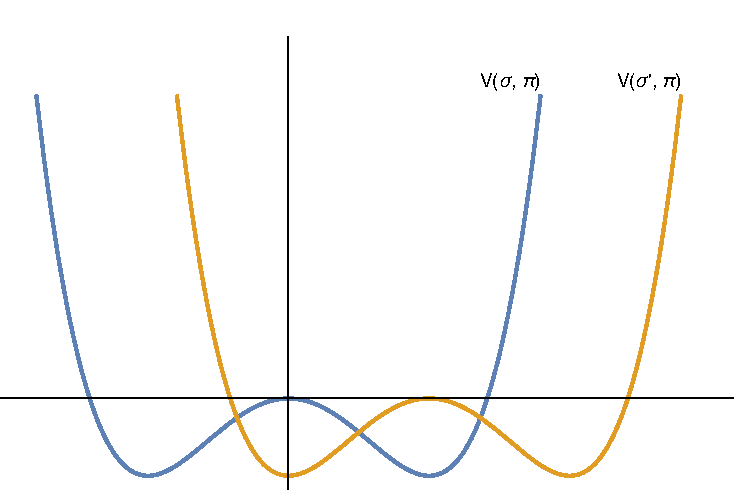
\includegraphics[scale=0.75]{shiftedpotential.pdf}
    \caption{Potential for $\sigma$ (blue) and $\sigma'$ (yellow).}
    \label{fig:shiftedpotential}
\end{figure}
Though the Lagrangian \eqref{lsmLagrangian} exibits ${S\!U}_L(2)\times {S\!U}_R(2)$ chiral symmetry, the ground state breaks this symmetry. Our Lagrangian in terms of our newly defined $\sigma'$ field is
\begin{align}
    \label{lsmLagrangianSSB}
      \mathcal{L} = & \bar{N}i \slashed{\partial}N + g\bar{N}(\sigma' + i \mathbf{\tau \cdot \pi}\gamma_{5})N + gv\bar{N}N\\ & +\frac{1}{2}\left[(\partial_{\mu}\mathbf{\pi})^{2}+(\partial_{\mu}\mathbf{\sigma'})^{2}\right]-\frac{1}{2}\mu^2\left({\sigma'}^2+\mathbf{\pi}^2\right) -\frac{1}{4}\lambda\left({\sigma'}^2+\mathbf{\pi}^2\right)^2\\
      & + (2v^2\lambda)\sigma'^2 + \mathrm{const.}
\end{align}
%CHECK THESE MASS RESULTS - Pokorski RESULT (p.237) IS DIFFERENT
Here we can observe a compelling property of the \lsm: the masses of the nucleon $N$ ($m_N = gv$) and the $\sigma'$ ($m_{\sigma'} = (2 v^2 \lambda)^(1/2)$) are dynamically generated through spontaneous chiral symmetry breaking, while the $\mathbf{\pi}$ Goldstone bosons remain massless (recall \eqref{lsmLagrangian} contained no explicit mass terms). This has similarities to the Anderson-Higgs mechanism which was later proposed \cite{higgs1,higgs2,higgs3} in that the introduction of a scalar particle dynamically generates a mass term through spontaneous symmetry breaking. In the case of the \lsm, this resolves simply with the generation of (in the chiral limit) Nambu-Goldstone bosons, while in the Anderson-Higgs mechanism the Nambu-Goldstone bosons provide mass to the $W^{\pm},\,Z$ gauge bosons. Given the role of the scalars in spontaneously breaking the chiral symmetry, this has motivated some to nominate the scalar mesons as the ``Higgs sector of the strong interaction'' \cite{Pennington2005,Schumacher2011}  despite the absence of an Anderson-Higgs mechanism.

To express the {\lsm} in terms of its chiral symmetry we can define a matrix field $\Sigma$ made up of our scalar and pseudoscalar fields
\begin{equation}
    \Sigma = \left(\sigma + i \tau \cdot \mathbf{\pi}\right)
    \label{lsm-matrix}
\end{equation}
where
\begin{equation}
    \sigma^{2} + \pi^{2} = \frac{1}{2}\Tr\left[\Sigma^{\dagger}\Sigma\right].
    \label{sigma-field}
\end{equation}
Using these results, as well as the properties of the chiral operators \eqref{chiralOperators}, we can express our {\lsm} Lagrangian \eqref{lsmLagrangian} in terms of $\Sigma$
\begin{equation}\label{lsmLagrangianMatrixForm}
\mathcal{L} = \bar{N}_{L}i \slashed{\partial}N_{L} + \bar{N}_{R}i \slashed{\partial}N_{R} + g\left( \bar{N}_{L}\Sigma N_{R} + \bar{N}_{R}\Sigma^{\dagger} N_{L} \right) + \frac{1}{4}\Tr\left[\partial_{\mu}\Sigma\partial^{\mu}\Sigma^{\dagger}\right] + \frac{1}{4} \mu^{2} \Tr\left[\Sigma^{\dagger}\Sigma\right] - \frac{\lambda}{16}\Tr\left[\Sigma^{\dagger}\Sigma\right]^{2}
\end{equation}
In this form, we can readily see the ${S\!U}_L(N_f)\times {S\!U}_R(N_f)$ chiral symmetry emerging, where our Lagrangian remains invariant under the transformation properties
\begin{gather}\label{su2Symmetries}
    N_{L,R} \rightarrow {N'}_{L,R} = g_{L,R} N_{L,R}\\
    \Sigma \rightarrow {\Sigma'} = U_{L}\Sigma U^{\dagger}_{R},
\end{gather}
where $g_{L,R} = \exp(-i \mathbf{\alpha}_{L,R}\cdot\mathbf{\tau}/2)$. Finally, the {\lsm} is frequently considered purely in the low-energy context as a description of pseudoscalar meson interaction; our equation \eqref{lsmLagrangianMatrixForm} is expressed in contemporary contexts as
\begin{equation}
    \mathcal{L}_{\mathrm{L\sigma M}} = \frac{1}{4}\Tr\left[\partial_{\mu}\Sigma\partial^{\mu}\Sigma^{\dagger}\right] + \frac{1}{4} \mu^{2} \Tr\left[\Sigma^{\dagger}\Sigma\right] - \frac{\lambda}{16}\Tr\left[\Sigma^{\dagger}\Sigma\right]^{2}.
    \label{lsmLagrangianMatrixForm-scalar}
\end{equation}

Efforts have been made since the discovery of quarks and the formalization of QCD to extend and modernize the {\lsm}, phrasing it instead in terms of constituent quarks \cite{Levy1967,Cabibbo1970,Delbourgo1995,Delbourgo1998}. However, it largely remains a toy model for exploring hadronic phenomena, and many are reluctant to refer to it as an effective theory of the strong interaction \cite{Donoghue1992,Ecker1994,Parganlija2017}. Several drawbacks of the {\lsm} are that the {\lsm} does not describe colour confinement, and the predictions of physical parameters in the theory deviate from those found experimentally \cite{Ecker1994}. For example, the dynamically generated nucleon mass $m_N = gv$ reflects a form of the Goldberger-Treiman relation
\begin{equation}
    \label{goldberger-treiman}
    g_{A} m_N = g_{\pi N N}f_\pi.
\end{equation}
As the pions are identified as pseudo-Nambu-Goldstone bosons, the vacuum expectation $v$ is identified with the pion decay constant $f_\pi$; further, our coupling $g = g_{\pi N N }$, which is apparent from its role in the nucleon-pion Lagrangian \eqref{lsmLagrangian}. The {\lsm} predicts a value in \eqref{goldberger-treiman} of $g_{A} = 1$, which is decidedly different from the measured experimental value of $g_{A} \approx 1.26$ \cite{PDG2018}.
Regardless of its shortcomings as an effective theory, the {\lsm} has provided an important foundation for our understanding of nucleon-pion interactions, the nature of the $\sigma$ meson, and to the mechanism of spontaneous symmetry breaking. It's usefulness in describing aspects of QCD give us compelling reasons to study it further as a model of the strong interaction. It has and it continues to provide a useful description of hadronic interaction, with some extending the model to include more hadronic states in attempts to explain the overpopulated scalar region \cite{Tornqvist2002,Parganlija2017, Fariborz2018} or including gauge fields to form a model of QCD \cite{Fariborz2009}.

\subsection{Nambu Jona-Lasino Model}
There are of course, other models of low-energy QCD that we will not delve into too much detail about, but nevertheless play an important role in the investigation of the scalar mesons. Much like the \lsm, the Nambu-Jona-Lasino model (NJLM) was proposed shortly after Gell-Mann and L\'evy's {\lsm} was published \cite{NJL1, NJL2}. Like the {\lsm}, the NJLM originally was a description of nucleon interactions, which has since been reinterpreted in the light of quarks and the formalism of QCD; it is an effective theory where gluonic degrees of freedom have been ``integrated out'' (see Section \ref{IV}). Because of this, not only do the bare quark masses ($\bar{m} = \frac{1}{2}(m_u + m_d) = 3.5\,\mev$ \cite{PDG2018}) appear in the NJLM, but \textit{constituent quark masses} ``dressed'' with information about the gluon dynamics also appear. These masses are considerably larger, and usually carry values similar to \cite{Schumacher2014}
\begin{gather}
    \label{constituent-quark-masses}
    m_u^{con} = 331\,\mev\\
    m_d^{con} = 335\,\mev.
\end{gather}

The Lagrangian for the NJLM is
\begin{equation}
    \label{njlm-lagrangian}
    \mathcal{L}_{\mathrm{NJLM}} = \bar{\psi}(i\slashed{\partial}-M)\psi + \frac{\lambda}{4}\left[ (\bar{\psi}\tau^{a}\psi)^{2}-(\bar{\psi}\gamma_{5}\tau^{a}\psi)^{2}\right] + K \left(\mathrm{det}\left[ \bar{\psi}(1+\gamma_5)psi\right] + \mathrm{det}\left[\bar{\psi}(1-\gamma_5)\psi\right]\right).
\end{equation}
The NJLM closely parallels the non-relativistic model of superconductivity by Bardeen, Cooper, and Schrieff; the four fermion interaction in \eqref{njlm-lagrangian} describes an attractive force between fermion pairs,  resulting in the creation of correlated Cooper pairs in BCS theory, while in the NJLM description this manifests as the chiral condensate $\langle \bar{q} q \rangle$ \cite{Hatsuda1994}. In the light of the NJLM, the chiral condensate is often interpreted as a condensation of quark-antiquark pairs in the vacuum, analogous to the Cooper-pair ground state in the BCS model of superconductivity \cite{Hatsuda1994}. The last term in \eqref{njlm-lagrangian} is called the \textit{'t Hooft interaction}, and was introduced to account for the broken $U_{A}(1)$ symmetry in QCD \cite{meissner1988nambu}.

A common approach to connect the quark-level NJLM to mesons is called \textit{bosonization} \cite{Ebert1998}, a formulation of the path-integral that approximates the quark-level terms with appropriate meson-level fields (i.e. $\bar{\psi}\tau^{a}\psi$ goes to a scalar field, $\bar{\psi}\gamma_{5}\tau^{a}\psi$ to pseudoscalar). In this way, the NJLM is well-suited to investigate the nature of the scalar nonet, much like the {\lsm} \cite{Hatsuda1994,BIJNENS1996370,Delbourgo1995}. In fact, the mass of the $\sigma$ meson is an important prediction of the NJLM \cite{Schumacher2014}, relating (in the chiral limit) $m_\sigma$ to the constituent quark mass $M$ by
\begin{equation}
    \label{sigma-mass}
    m_\sigma = 2M \approx 652\,\mev.
\end{equation}

\section{Non-linear $\sigma$ Model}\label{IV}
In Gell-Mann and L\'evy's original work \cite{GellMann1960}, the {\lsm} was proposed as a model of pion-nucleon interactions. However, the preservation of ${S\!U}_L(N_f)\times {S\!U}_R(N_f)$ symmetry required the addition of the isoscalar $\sigma$, which at the time had been predicted \cite{Schwinger1957}, but not experimentally observed. Perhaps concerned about this, Gell-Mann and L\'evy carried their model further and, by making use of the spontaneous chiral symmetry breaking in the {\lsm} and the non-zero VEV described by \eqref{doublewellMinimum}, and eliminate the $\sigma$ field by the constraint
\begin{equation}
    \label{nlsm-condition}
    \sigma = \sqrt{v^2 - \mathbf{\pi}^2}.
\end{equation}
From here, our transformations \eqref{lsm-vectortransformations} and \eqref{lsm-axialvectortransformation} become
\begin{gather}
    \pi   \rightarrow \pi + \alpha_V \times \pi \label{nlsm-vector}\\
    \pi   \rightarrow \pi + \alpha_A \sqrt{v^2 - \mathbf{\pi}^2}\label{nlsm-axial}.
\end{gather}
The Lagrangian can be expressed using our previously defined matrix field \eqref{sigma-field}, our constraint \eqref{nlsm-condition}, and enforcing unitarity such that
\begin{equation}
    \label{nlsm-matrix-field}
    U = \frac{1}{v}\left( \sqrt{v^2 - \mathbf{\pi}^2} + i \tau \cdot \mathbf{\pi}\right).
\end{equation}

This modification to the {\lsm} is known as the non-linear $\sigma$ model (\nlsm), as the $\sigma$ field has been exchanged for a nonlinear transformation in \eqref{nlsm-axial}. Substituting \eqref{nlsm-matrix-field} into \eqref{lsmLagrangianMatrixForm-scalar}, we get
\begin{equation}
    \label{nlsm-lagrangian}
    \mathcal{L}_{\mathrm{NL\sigma M}} = \frac{v^2}{4}\Tr \left [ (\partial_{\mu} U)(\partial_{\mu} U)^\dagger\right],
\end{equation}
where the other terms in \eqref{lsmLagrangianMatrixForm-scalar} have just become constant terms and therefore not included. Coincidently, this is also the simplest term that we can write down from a unitary matrix $U$ that respects the necessary $S\!U(N_f)$ symmetry. However, \eqref{nlsm-matrix-field} is not a unique parameterization, and others may be found in the literature provided the symmetries are fulfilled. It is common when discussing the nonet of pseudoscalars within both the {\lsm} and {\nlsm} models to define 
\begin{gather}
    \label{pseudoscalar-matrix1}
    U = \exp (\frac{i \sqrt{2}}{f_\pi}\Phi)\\
    \mathrm{where}\,
    \Phi =  \begin{pmatrix}
          \frac{1}{\sqrt{2}}\pi^{0}+\frac{1}{\sqrt{6}}\eta & \pi^{+} & K^{+} \\
          \pi^{-} & -\frac{1}{\sqrt{2}}\pi^{0}+\frac{1}{\sqrt{6}}\eta & K^{0} \\
          K^{-} & \bar{K}^{0} & -\frac{2}{\sqrt{6}} \eta  \label{pseudoscalar-matrix2}
        \end{pmatrix}
\end{gather}


Since the $\sigma$ meson was first suggested by Schwinger \cite{Schwinger1957}, the particle has had a controversial history, and as its status as a real particle has shifted, so have the models and tools used to investigate. The {\lsm} has explicitly built into it a prediction about the $\sigma$, while the {\nlsm} explicitly integrates it out. The {\nlsm} has been utilized in a wide variety of topics ranging from its original intended use of investigating hadronic physics and the strong interaction \cite{GellMann1960}, to condensed matter \cite{nlsm-condmat1,nlsm-condmat2}, and supersymmetric theories \cite{Bagger1984,Witten1988}. We will next investigate how it forms the foundation of a prolific effective field theory of the strong interaction.

\subsection{Chiral Perturbation Theory}
In an effort to better understand complicated physical phenomena in particle physics, effective field theories (EFTs) have been an important tool for approximating sophisticated, unknown, or incomplete theories. Effective theories are built based on a specific range of distance or energy scales that are to be explored; just as quantum mechanics is not necessary to calculate the period of a simple pendulum, EFTs need not be comprehensive explanations of phenomena. They have been of particular use in exploring QCD and the strong interaction. The non-abelian nature of QCD makes it a challenge to calculate processes, particularly at higher orders of expansion and at energies outside of the perturbative regime. There are many effective theories commonly in use which describe different aspects of the strong interaction, such as
\begin{itemize}
    \item Heavy Quark Effective Theory (HQET)
    \item Non-relativistic QCD (NRQCD)
    \item Soft collinear Effective theory (SCET)
    \item Chiral Perturbation Theory ($\chi$PT)
\end{itemize}
Of these EFTs, HQET and NRQCD address hadronic systems containing heavy-flavoured quarks ($c$ or $b$ quarks), and SCET describes interactions between hard and soft processes. We restrict our study to $\chi$PT, which pertains to light systems and low-energy hadronic phenomena. 

In an effective theory, because we generally are only interested in physics at a particular energy scale, heavier particles are removed from consideration. The decoupling theorem says,
\begin{quote}
    \textit{...if the remaining low-energy theory is renomalizable, then all effects of the heavy-particle appear either as a renormalization of the coupling constants in the theory, or else are suppressed by powers of the heavy-particle mass.}
\end{quote}
as stated by Donoghue \cite{Donoghue1992}. Given that propogators appear as powers of $1/M$, if we consider a particular energy region where the particles of interest have a mass much less than those at higher energies, we can consider these heavy particle masses as infinitely large. This is referred to as ``integrating out'' the fields, coming from the path integral treatment of forming an effective action by integrating over all heavy particles, resulting in an overall constant in our path integral.

From the principles of effective field theory and the symmetries of QCD, {\cpt} emerges as a framework for systematically exploring low-energy QCD. In traditional \cpt, the particles which are significant degrees of freedom at the relevant energy scales are the pions, the kaons, and the $\eta$; particles belonging to the pseudoscalar multiplets can be separated from the rest of the hadrons thanks to the mass gap caused by spontaneous symmetry breaking. We can build our effective theory from the framework of our {\lsm}; we consider pions (pseudo-Nambu-Goldstone bosons) to be much lighter than the $\sigma$ degrees of freedom in the {\lsm}. To build an effective theory, we must write down all terms which obey the symmetries that we wish to consider, in our case the ${S\!U}_L(N_f)\times {S\!U}_R(N_f)$ chiral symmetry expected from QCD in the limit of massless quarks. If we consider all the pseudoscalars in matrix form as in \eqref{pseudoscalar-matrix1} and \eqref{pseudoscalar-matrix2}, the lowest-order contribution to our chiral Lagrangian that can be realized corresponds to our {\nlsm} Lagrangian \eqref{nlsm-lagrangian} (in other words, to lowest order the Lagrangian of {\cpt} takes the same form of a {\lsm} with the scalar ``integrated out''). In fact, if we simply build the most general Lagrangian invariant under ${S\!U}_L(N_f)\times {S\!U}_R(N_f)$ for $N_f \times N_f$ unitary matrix $U$ (in the absence of external fields),
\begin{align}
    \label{cpt-lagrangian-massless}
    \mathcal{L}_{\chi PT} = & \frac{f_{\pi}^{2}}{4} \tr \left[(\partial_{\mu} U)(\partial_{\mu} U)^{\dagger}\right] + L_{1} \tr \left[(\partial_{\mu} U)(\partial_{\mu} U)^{\dagger}\right]^{2} \\
    & + L_{2}\tr \left[(\partial_{\mu} U)(\partial_{\nu} U)^{\dagger}\right]\tr \left[(\partial_{\nu} U)(\partial_{\mu} U)^{\dagger}\right] \\
    & + L_{3} \tr \left[(\partial_{\mu} U)(\partial_{\mu} U)^{\dagger}(\partial_{\nu} U)(\partial_{\nu} U)^{\dagger} \right] + \ldots
\end{align}
Here, the coefficients $L_i$ are \textit{low-energy constants} (LECs) that represent the underlying dynamics that the effective field theory describes; they can be considered as couplings or interaction vertices. In a sense, these LECs represent contributions from higher energies that have been integrated out of the Lagrangian. Usually the values of these LECs are not known, and must be found by fitting to experimental results \cite{Gasser1984,Bijnens2014}; while progress has been made in calculating LECs on the lattice, the results are still not competitive when compared to traditional methods. \cite{Bijnens2014}.
To generalize \eqref{cpt-lagrangian-massless} to include external fields, we can promote $\partial_\mu \rightarrow D_\mu$ where
\begin{equation}
    \label{covariantDerivativedefn}
    D_\mu U = \partial_\mu U + i l_\mu - i r_\mu,
\end{equation}
and the resulting field-strength tensors are defined analogously to gauge fields,
\begin{gather}
    \label{fieldstrengthTensor1}
    L_{\mu\nu} = \partial_\mu l_\nu - \partial_\nu l_\mu + i \left[l_\mu,l_\nu\right]\\
    \label{fieldstrengthTensor2}
    R_{\mu\nu} = \partial_\mu r_\nu - \partial_\nu r_\mu + i \left[r_\mu,r_\nu\right].
\end{gather}
These must have the correct chiral symmetry transformations,
\begin{gather}
    \label{fieldTransformations}
    l_\mu \rightarrow L(x) l_\mu L^\dagger(x) + i\partial_\mu L(x)L^\dagger(x)\\ 
    r_\mu \rightarrow R(x) r_\mu R^\dagger(x) + i\partial_\mu R(x)R^\dagger(x)\\
    L_{\mu\nu} \rightarrow L(x) L_{\mu\nu} L^\dagger(x)\\
    R_{\mu\nu} \rightarrow R(x) R_{\mu\nu} R^\dagger(x),
\end{gather}
where $L,\,R$ are in $S\!U(N_f)$. In this formalism, we can include external fields in our calculations.

We know that chiral symmetry is explicitly broken by the quark masses; however, effective field theories are built around symmetric Lagrangians. To explore the effect that quark masses have on the masses of the pseudoscalars while preserving the necessary ${S\!U}_L(N_f)\times {S\!U}_R(N_f)$ symmetry for the effective theory, we can define a mass matrix
\begin{equation}
    \label{mass-matrix}
    M = \begin{pmatrix}
            m_{u} & 0 &0 \\
            0 & m_{d} & 0 \\
            0 & 0     & m_{s} 
        \end{pmatrix},
\end{equation}
and assign the transformation $M \rightarrow g_L M g^{\dagger}_{R}$, making it invariant under $\groupsu{3}$. From this, we can add the ${S\!U}_L(N_f)\times {S\!U}_R(N_f)$ invariant term
\begin{equation}
    \label{cpt-massterm}
    \mathcal{L}_{M} = \frac{V^{3}}{2}\tr \left[MU + M^{\dagger}U^{\dagger} \right],
\end{equation}
where $U$ is defined in \eqref{pseudoscalar-matrix1} and \eqref{pseudoscalar-matrix2}. Expanding $U$ out to $\mathcal{O}\left(\Phi^2\right)$ and working out \eqref{cpt-massterm}, we find mass terms generated in the Lagrangian for each set of mesons described in \eqref{pseudoscalar-matrix2}, and can assign
\begin{gather}
    m_\pi^{2} = \frac{V^3}{f_\pi^{2}}(m_u + m_d) \label{GMOR2}\\
    m_{K^{\pm}}^{2} = \frac{V^3}{f_\pi^{2}}(m_s + m_u)  \\
    m_{K^{0}}^{2} = \frac{V^3}{f_\pi^{2}}(m_s + m_d)  \\
    m_{\eta}^{2} = \frac{V^3}{3f_\pi^{2}}(4m_s + m_u + m_d). 
\end{gather}
A quick calculation shows that these first-order calculations are good estimates of the pseudoscalar masses; from the above relationships we can write
\begin{equation}
    m_\eta^{2} = \frac{1}{3}\left( 2\left(m^2_{K^0}+m^2_{K^\pm}\right) - m_\pi^{2} \right)
\end{equation}
Using PDG values \cite{PDG2018} of $m_{K^\pm}=497.6\,\mev$, $m_{K^0}=493.7\,\mev$, and $m_{\pi}=135\,\mev$, we find a predicted $\eta$ mass of $m_\eta = 567\,\mev$, with its measured mass being slightly less at $m_\eta^{\mathrm{PDG}} = 547.9\,\mev$. Further, we notice that \eqref{GMOR2} is simply the GMOR relation \eqref{GMOR}, and we can see that $V^3$ simply relates to the chiral condensate $\langle \bar{q}q\rangle$. Thus, we can write the lowest order chiral Lagrangian for {\cpt} as
\begin{equation}
    \label{cpt-Langrangian-LO}
    \mathcal{L}_{\chi PT} = \frac{f_{\pi}^{2}}{4} \tr \left[(\partial_{\mu} U)(\partial_{\mu} U)^{\dagger}\right]-\frac{\langle \bar{q}q\rangle}{4}\tr \left[MU + M^{\dagger}U^{\dagger} \right].
\end{equation}
The LECs for {\cpt} in the context of the light mesons is known well up to NLO ($\mathcal{O}\left(p^4\right)$), with promising precision at NNLO ($\mathcal{O}\left(p^6\right)$) \cite{Bijnens2014} for $N_f = 2$ and $N_f = 3$. They are determined from processes such as $\pi\pi$/$\pi K$ scattering data and $K\rightarrow \pi\pi\pi$ decays, as well as from parameters including hadron and quark masses, and coupling constants.

Modifications to the framework have been used to explore the vector mesons \cite{Bijnens1997}, tensor mesons \cite{Chow1998}, and baryons \cite{Bernard2008}; in these cases, typically another methodology such as large $N_c$ expansion is used to estimate the values of the LECs at the new energy scale. However, moving beyond tree-level calculations introduces divergences that historically stalled progress in {\cpt} until an appropriate renormalization procedure was proposed \cite{Gasser1984}. While {\cpt} is a non-renormalizable theory in the traditional sense (at sufficient orders of perturbative expansion, the LECs have negative mass dimension), it was proposed that renormalization be done order-by-order by adding the relevant counterterms needed to cancel divergences. While this theoretically means that there exists an infinite number of counterterms in {\cpt}, in practice one simply expands to the order of interest based on the relevant energy scale \cite{Gasser1984,Donoghue1992,Holstein2000}. 

\section{Investigating the structure of the scalar nonet}\label{V}
\subsection{Linear Sigma Model Applications}
While the {\lsm} had fallen out of favour with the uncertainty of the experimental status of the $\sigma$ meson \cite{Ecker1994}, literature following the confirmation of the $\sigma$ resonance \cite{Tornqvist1996} seems to indicate a return to the model given its direct tie to the scalar mesons. Since then, there have been many generalizations of the {\lsm} in hopes that it might shed light on the nature of the scalar mesons discussed in Section \ref{II}, glueballs, as well as the restoration of chiral symmetry \cite{Delbourgo1995,Delbourgo1998,Lenaghan2000,Fariborz2018}. In general, investigations into the nature of the scalar nonet begin with the Lagrangian \eqref{lsmLagrangianMatrixForm-scalar} plus extensions (for example, gauge bosons \cite{Fariborz2009}, other nonets \cite{Parganlija2017}, or glueballs \cite{Fariborz2018}), and define a matrix form for $\Sigma$ corresponding to the orthogonal scalar states analogous to \eqref{lsm-matrix}. For example, in investigating the scalar states in the context of radial excitations in an extended {\lsm}, Ref. \cite{Parganlija2017} defines the scalar ($S_i$) and pseudoscalar ($P_i$) nonet through the appropriate group generators $T_i$ as
\begin{gather}
   \Sigma =  (S_i + i P_i)T_i = \frac{1}{\sqrt{2}}\begin{pmatrix}
          \frac{1}{\sqrt{2}}((\sigma_N + a_0^0)+i(\eta_N + \pi^0)) & a_0^{+}+i\pi^{+} & K^{*+}_0 + iK^{+} \\
          a_0^{-}+i\pi^{-} & \frac{1}{\sqrt{2}}((\sigma_N - a_0^0)+i(\eta_N - \pi^0)) & K^{*0}_0 + iK^{0} \\
           K^{*-}_0 + iK^{-} & \bar{K}^{*0}_0 + i\bar{K}^{0} & \sigma_S + i \eta_S  \label{scalar-matrix2},
        \end{pmatrix}
\end{gather}
as well as similar matrices for the vector nonets. 
Conclusions from studies using {\lsm} methods appear to be unclear. Though utilizing the same initial Lagrangian, four separate groups come to four drastically different results for the mass of the $\sigma$ and $\kappa$ \cite{Napsuciale1998, Napsuciale2001,Tornqvist1999,tHooft2008,Black2001}, which could be a result of insufficient experimental parameters to constrain the models \cite{Bramon2004}.  

We can compare the prediction power of the {\lsm} against {\cpt} by comparing LECs from both theories; by integrating out the $\sigma$ from the {\lsm}, we form LECs which we can compare to those in {\cpt} obtained from fitting to experiment. What we find is that while the {\lsm} and {\cpt} may have similar predictions at leading order, the LECs derived from the {\lsm} deviate from the LECs from {\cpt} at NLO. Many indicate that this implies the {\lsm} does not carry the correct description of physics for a low energy effective theory of QCD \cite{Donoghue1992,Pelaez2011}. However, others have suggested that investigating the compatibility between the {\lsm} and {\cpt} could allow deeper insight into the dynamics of the scalar mesons, given the scalars are addressed explicitly by the {\lsm}, while the dynamics of the scalars are hidden in the LECs of {\cpt} \cite{Tornqvist1999,Bramon2004}. It is also worth acknowledging that {\cpt} and the {\lsm} are anchored at distinct energies; {\cpt} to the pseudoscalars, and the {\lsm} to the scalars. This could account for the deviation in the LECs \cite{Tornqvist1999}, and in fact it is found that the {\lsm} is consistent with {\cpt} if restricted to LECs generated by scalar resonances \cite{Bramon2004}.

While often looked over as simply a ``toy model'', a significant amount of research has gone into turning the {\lsm} into a viable phenomenological model \cite{Napsuciale1998, Napsuciale2001,Tornqvist1999,tHooft2008,Black2001,Scadron2013,Fariborz2018}. It shows promise as a way of explicitly incorporating a scalar nonet into low-energy QCD, and captures the appropriate symmetries needed to describe the strong interaction. However, more precise experimental data on the scalars and a better understanding of the relationship between the {\lsm} and {\cpt} is necessary to distinguish the {\lsm} as a predictive model in its own right.

\subsection{Non-linear Sigma Model and Chiral Perturbation Theory}  
Fully established as a predictive theory in the mid 1980s \cite{Gasser1984}, {\cpt} has become popularized as the ``correct'' description of low-energy QCD, though that this is the only correct description remains disputed by some researchers \cite{Tornqvist1999}. Because of its success in predicting low-energy phenomena (and perhaps in part because of its silence on the controversial $\sigma$ meson and its popularization during an era where the $\sigma$ was experimentally tenuous), {\cpt} has become a standard methodology in investigating low-energy phenomena. It has seen many predictions successfully confirmed by experiment, such as pion polarizabilities \cite{Scherer2006}, $\pi\pi$ scattering, and $\pi$ production \cite{Merkel2004}.

Given some properties of what are predicted to be the scalar quarkonia mesons are difficult to describe in a pure $q\bar{q}$ paradigm, it has been suggested that mixing between a glueball, a four-quark and a quarkonia scalar nonet could be responsible for the deviation from the $q \bar{q}$ picture\cite{Fariborz2003}. This model is consistent with a four-quark $f_0(500)$ state as well as a scalar glueball mass of $\approx 1.47-1.64 \,\gev$, with significant glueball content predicted for the $f_0(1500)$ and $f_0(1710)$ states. Other treatments within a {\cpt} framework have obtained similar predictions for the large gluonic component of $f_0(1500)$ and $f_0(1710)$ states with minimal mixing between scalar nonets \cite{Giacosa2005}. 
Calculations of the scalar nonet have been done in {\cpt} to $\mathcal{O}(p^2)$ considering the scalars as diquark-molecular structures \cite{Xiao2008}. 

Due to its reliability at lower energy scales, {\cpt} has become a valuable tool for practitioners of lattice QCD. By quantizing spacetime, the method aims to solve the path integral equations without introducing models and minimizing approximations. Doing so takes compromise; discretizing spacetime destroys underlying continuous symmetries including Lorentz and chiral symmetry, which is nontrivial to restore \cite{walecka2004}. Reestablishing chiral symmetry in lattice gauge theories has long been possible \cite{DeGrand2007}, however it remains that simulations done at small lattice spacings small enough take enormous computing resources reserved for collaborations with adequate resources \cite{Jansen2013}. Lattice practitioners have often used {\cpt} as a ways to extrapolate down to lower energy scales. As lattice simulations have become more and more sophisticated, they have also been able to calculate LECs within {\cpt} \cite{Aoki2019}. Regarding the scalar nonet, lattice studies have begun probing the structural nature of the scalar nonets and the identity of the scalar glueball \cite{Lee:1999kv,McNeile:2000xx,Alford:2000mm,WADA2004432,Mathur2007}. Several studies have come out in favor of a tetraquark/mesonium interpretation for low-lying scalar states (e.g. the $f_0(500)$, $f_0(980)$, $a_0(980)$, or $K^{*}(700)$)\cite{Alford:2000mm,Mathur2007}, though recent lattice simulations claim little to no tetraquark content in the $a_0(980)$ or $K^{*}(700)$ states \cite{Wagner2013}, both commonly claimed as belonging to a scalar four-quark nonet \cite{Pennington2005,Pelaez2011,Schumacher2011}. As these states exist in the realm of low-energy QCD where the effects of chiral symmetry breaking are unquestionably important, it is likely that clear predictions as to the nature of the scalar mesons from lattice QCD will require robust simulations at small quark masses, with dynamic quarks, and contributions from disconnected diagrams \cite{WADA2004432,McNeile:2007qf,Mathur2007}.

Investigation of the scalar mesons in both the {\lsm} and {\cpt} prove challenging due to the uncertainty and controversy in the classification of the scalar nonet. More precise experimental data is needed to refine descriptions of QCD in {\cpt}.

\section{Conclusion}
Important questions about the nature of matter and the strong interaction are still unanswered at the low end of high-energy physics. While there are many theoretical tools available to probe these regions, more experimental results are needed to better confine models, and provide a cleaner picture of the dynamics at play at these energies. While computational tools such as lattice QCD are making some progress, models and effective theories still remain important methodologies for exploring low-energy regimes. The linear $\sigma$ models and non-linear $\sigma$ models form influential categories of models that have left their mark on many different areas of physics, yet still remain important and influential in their original applications of the strong interaction. There have been strong efforts to investigate the properties of the scalar meson multiplet utilizing both methodologies. The experimental nature of the lowest-lying scalar states remain unclear, with states like the $f_0(500)/\sigma$ meson being especially controversial over the past six decades. Strong evidence has emerged for a nonet composed of the $f_0(500)$, $f_0(980)$, $a_0(980)$, and the $K^{*}_0(700)$, both from experiment and theory. However the literature is far from consensus regarding the nature of these states, with some identifying them as four-quark states (tightly or loosely bound), conventional $q\bar{q}$ states, or glueball states. It is clear that more precise experimental data is necessary to confirm the existence of some of the more experimentally precarious scalar resonances, to clarify the identity of the scalar glueball, and to further constrain the models used to investigate the structure of the scalar multiplet. 
\clearpage
%\bibliographystyle{h-physrev}
\bibliography{research}

\end{document}